

\StartOf{Lecture 2}

\Today{ (1) Power, Energy, dB, (2) Orthogonality, (3) Periodicity and Impulse Functions}

%\announcements{}

\section{Power and Energy}


Two of the biggest limitations in communications systems are (1) \textit{energy} / \textit{power}; and (2) \textit{bandwidth}.  This section provides some tools to deal with power and energy.


Recall that energy is power times time.  \textbf{Use the units}:  energy is measured in Joules (J); power is measured in Watts (W) which is the same as Joules/second (J/sec).  Also, recall that our standard in signals and systems is define our signals, such as $x(t)$, as voltage signals (V).  When we want to know the power of a signal we assume it is being dissipated in a 1 Ohm resistor, so $|x(t)|^2$ is the power dissipated at time $t$ (since power is equal to the voltage squared divided by the resistance).  The actual received power a

A signal $x(t)$ has energy defined as
\[
E = \int_{-\infty}^\infty |x(t)|^2 dt
\]
A signal with finite energy is called a \emph{waveform} or \emph{energy signal}.  
For some signals, $E$ will be infinite because the signal is
non-zero for an infinite duration of time (it is always on).  These
signals we call {\it power signals} and we compute their power as
\[
  P = \limin{T} \frac{1}{2T} \int_{-T}^T |x(t)|^2 dt
\]



\subsection{Discrete-Time Signals}

In the Rice book, we refer to discrete samples of the sampled signal $x$
as $x(n)$.  You may be more familiar with the $x[n]$ notation.  But,
Matlab uses parentheses also; so we'll follow the Rice text
notation.  Essentially, whenever you see a function of $n$ (or $k$, $l$, $m$), it is a discrete-time function; whenever you see a function of $t$ (or perhaps $\tau$) it is a continuous-time function.  I'm sorry this is not more obvious in the notation.

For discrete-time signals, energy and power are defined as:
\begin{eqnarray}
  E &=& \sum_{n=-\infty}^\infty |x(n)|^2 \\
  P &=& \limin{N} \frac{1}{2N+1} \sum_{n=-N}^N |x(n)|^2
\end{eqnarray}


\subsection{Decibel Notation}

We often use a decibel (dB) scale for power.  If $P_{lin}$ is the
power in Watts, then the power in dBW is
\[
  \dBW{P} = 10 \log_{10} \frac{P_{lin}}{1 \mbox{ W}}.
\]
We convert from dB to linear by inverting the above formula,
\[
  P_{lin} = (1 \mbox{ W}) 10^{\dBW{P}/10} .
\]

Decibels are more general - they can apply to other unitless
quantities as well, such as a gain (loss) $L(f)$ through a filter
$H(f)$,
\begin{equation} \label{E:filterGaindB}
  \dB{L(f)} = 10 \log_{10} |H(f)|^2
\end{equation}

Note: Why is the capital B used?  The `Bel' refers to a Alexander Graham
`Bell' so it is capitalized.  The Bel is defined as the $\log_{10}$ of the ratio, so following the SI convention, the decibel is ten times that. The standard is to use the
decibel $10 \log_{10} (\cdot)$ which is then abbreviated as dB, just like milliwatt is abbreviated mW in the SI system.

Note that (\ref{E:filterGaindB}) could also be written as:
\begin{equation} \label{E:filterGaindB2}
  \dB{L(f)} = 20 \log_{10} |H(f)|
\end{equation}
Be careful with your use of 10 vs.~20 in the dB formula.  
\begin{itemize}
 \item Only use 20 as the multiplier if you are converting from voltage to power; \ie, taking the $\log_{10}$ of a voltage and expecting the result to be a dB power value.
\end{itemize}

Our standard is to consider power gains and losses, not voltage gains and losses.  So if we say, for example, the channel has a loss of 20 dB, this refers to a loss in power.  In particular, the output of the channel has 100 times less power than the input to the channel.

Remember these two dB numbers:
\begin{itemize}
  \item 3 dB:  This means the number is double in linear terms.
  \item 10 dB:  This means the number is ten times in linear terms.
\end{itemize}
And maybe this one:
\begin{itemize}
  \item 1 dB:  This means the number is a little over 25\% more (multiply by 5/4) in linear terms.
\end{itemize}
With these three numbers, you can quickly convert losses or gains between
linear and dB units without a calculator.  Just convert any dB number into a sum of multiples of 10, 3, and 1.

\Example{Convert dB to linear values:}
\begin{enumerate}
 \item 30 dBW
 \item 33 dBm
 \item -20 dB
 \item 4 dB
\end{enumerate}
\Solution{
\begin{enumerate}
 \item $(1 \mbox{ W}) 10^{\dBW{30}/10} = 10^3 \mbox{W} = 1000$ W.
 \item 33 dBm = 30 dBm + 3 dB = 1000 mW $\times 2$ = 2 W.
 \item -20 dB = $10^{\dBW{-20}/10} = 10^{-2} = 0.01$.
 \item 4 dB = 3 dB + 1 dB $\approx 2(1.25) =2.5$.
\end{enumerate}
}

\Example{Convert linear values to dB:}
\begin{enumerate}
 \item 0.2 W
 \item 40 mW
\end{enumerate}
\Solution{
\begin{enumerate}
 \item 0.2 W $= (0.1 \mbox{W})(2) = \dBW(-10) + \dB{3} = -7$ dBW
 \item 40 mW $= (10 \mbox{mW})(2)(2) = \dBm{10} + \dB{3} + \dB{3} = \dBW{16}$.
\end{enumerate}
}
\Example{Convert power relationships to dB:}  Convert the expression to one which involves only dB terms.
\begin{enumerate}
 \item $P_{y,lin} = 100 P_{x,lin}$
 \item $P_{o,lin} = G_{connector,lin} L_{cable,lin}^{-d}$, where $P_{o,lin}$ is the received power in a fiber-optic link, where $d$ is the cable length (typically in units of km), $G_{connector,lin}$ is the gain in any connectors, and $L_{cable,lin}$ is a loss in a 1 km cable.
 \item $P_{r,lin} = P_{t,lin} \frac{G_{t,lin} G_{t,lin} \lambda^2}{(4\pi d)^2}$, where $\lambda$ is the wavelength (m), $d$ is the path length (m), and $G_{t,lin}$ and $G_{t,lin}$ are the linear gains in the antennas, $P_{t,lin}$ is the transmit power (W) and $P_{r,lin}$ is the received power (W).  This is the Friis free space path loss formula.
\end{enumerate}

These last two are what we will need in Section 6.4, when we discuss link budgets.  The main idea is that we have a limited amount of power which will be available at the receiver.



\section{Orthogonality}
In the introductory lecture, we described a couple reasons why orthogonal signals are used in digital communication systems.  In short, we use orthogonal signals for:
\begin{enumerate}
 \item \emph{Multiple Access}: Multiple users can access the same medium, and a receiver can separate one user's signal from the rest.
 \item \emph{Increasing Signal Dimension}: A single user can send information along multiple dimensions at the same time, which is useful for increasing the bit rate or fidelity.
\end{enumerate}

Also, I gave  my ``engineering'' definition of a set of orthogonal waveforms:  \emph{They are waveforms that can be separated at the receiver.}  Now, let's provide the mathematical definition.

\Definition{Orthogonal}{  Two real-valued waveforms $\phi_0(t)$ and $\phi_1(t)$ are
\textit{orthogonal} if
\[
  \int_{-\infty}^\infty \phi_0(t)\phi_1(t) dt = 0.
\] 
Two complex-valued waveforms $\phi_0(t)$ and $\phi_1(t)$ are orthogonal if
\[
  \int_{-\infty}^\infty \phi_0(t) \phi_1^*(t) dt = 0,
\] 
where $\phi_1^*(t)$ is the complex conjugate of $\phi_1(t)$.
}

What does this integral remind you of?

\Definition{Orthogonal Set}{$K$ waveforms $\phi_0(t), \ldots, \phi_{K-1}(t)$ are
mutually orthogonal, or form an orthogonal set, if every pair of waveforms $\phi_i(t)$, $\phi_j(t)$, for $i\neq j$, is orthogonal.}

\Example{Sine and Cosine} Let
\begin{eqnarray}
 \phi_0(t) &=& \pdfarray{\cos(2\pi t)}{0< t \le 1} \nonumber \\
 \phi_1(t) &=& \pdfarray{\sin(2\pi t)}{0< t \le 1} \nonumber
\end{eqnarray}
Are $\phi_0(t)$ and $\phi_1(t)$ orthogonal?

\Solution{
Using $\sin 2x = 2 \cos x \sin x$, 
\begin{eqnarray}
  \int_{-\infty}^\infty \phi_0(t)\phi_1(t) dt  &=& \int_0^1 \cos(2\pi t)\sin(2\pi t)dt  \nnn
   &=&\int_0^1 \frac{1}{2}\sin(4\pi t)dt \nnn
   &=& \left. \frac{-1}{8\pi}\cos(4\pi t)\right|_0^1 = \frac{-1}{8\pi}(1-1) = 0  \nn
\end{eqnarray}
So, yes, $\phi_0(t)$ and $\phi_1(t)$ are orthogonal.
}

\Example{Frequency Shift Keying}  Assume $T_s >> 1/f_c$, and show that these two are orthogonal.
\begin{eqnarray} \label{E:FSK-Symbols}
 \phi_0(t) &=& \pdfarray{\cos \left(2\pi f_c t  \right)}{0 \le t \le T_s} \nnn
 \phi_1(t) &=& \pdfarray{\cos \left( 2\pi \left[f_c + \frac{1}{T_{s}}\right] t \right)}{0 \le t \le T_s} \nn
\end{eqnarray}

\Solution{ The integral of the product of the two must be zero.  Checking, and using the identity for the product of two cosines,
\begin{eqnarray} \label{E:FSK-Symbols2}
 && \int_0^{T_s} \cos \left(2\pi f_c t  \right) \cos \left( 2\pi \left[f_c + \frac{1}{T_{s}}\right] t \right)  dt
\nnn
 &=& \frac{1}{2}\int_0^{T_s} \cos \left(2\pi t/T_s  \right) dt + \frac{1}{2} \int_0^{T_s} \cos \left( 4\pi f_c t + 2\pi t/T_{s} \right)  dt
\nnn
 &=& 0 + \frac{1}{2}\left[ \frac{1}{2 \pi (2f_c + 1/T_s)} \sin \left( 2\pi ( 2 f_c + 1/T_{s}) t \right) \right|_0^{T_s}  
\nn
\end{eqnarray}
The remaining term has a $\frac{1}{2 \pi (2f_c + 1/T_s)}$ constant out front.  Because $f_c$ is very high, this term will be very very low.  The sine term is limited to between -1 and +1 so it will not cause the second term to be large.  Thus,
\begin{eqnarray} \label{E:FSK-Symbols3}
\int_{-\infty}^\infty \phi_0(t)\phi_1(t) dt   \le  \frac{1}{ \pi (2f_c + 1/T_s)} &\approx&  0
\nn
\end{eqnarray}
Thus the two different frequency waveforms are orthogonal.
}

\subsection{Linear Combinations}

What is a linear combination of orthogonal waveforms?  Well, consider the orthogonal set $\phi_0(t), \ldots, \phi_{K-1}(t)$.  A linear combination $s_m(t)$ is
\[
 s_m(t) = a_{m,0} \phi_0(t) + a_{m,1} \phi_1(t) + \cdots + a_{m,K-1} \phi_{K-1}(t) = \sum_{m=k}^{K-1} a_{m,k} \phi_k(t)
\]
We also call the a linear combination a {\it symbol}.  We use subscript $m$ to indicate that it's not the only possible linear combination (or symbol).  In fact, we will use $M$ different symbols, so $i=0, \ldots, M-1$, and we will use $s_0(t), \ldots, s_{M-1}(t)$.

We represent the $m$th symbol (linear combination of the orthogonal waveforms), $s_m(t)$, as a vector for ease of notation:
\[
\mbs_m = [a_{m,0}, a_{m,1}, \ldots, a_{m,K-1}]^T 
\]
The superscript $T$ is for transpose -- $\mbs_m$ is a column vector.  Vectors are easy to deal with because they can be plotted in vector space, to show graphically what is going on.  We call the plot of all possible $\mbs_m$, that is, for $m=0, \ldots M-1$, the \textit{constellation diagram}.  Some examples are shown in Figure \ref{F:MPSKEg}.


\subsection{Using $M$ Different Linear Combinations}

Here is how a transmitter \emph{uses} the different linear combinations to convey digital bits to the receiver.  First, consider that there are $M$ different symbols for the TX to chose from.  Each symbol is described by a $\log_2 M$-length bit sequence.  For example, if there are $8$ possible combinations, we would label them 000, 001, 011, 010, 110, 111, 101, 100.  

The transmitter knows which $\log_2 M$-bit sequence it wants to send.  It picks the symbol that corresponds to that bit sequence, let's call it symbol $m$.  Then it sends $s_m(t)$.  

If the receiver is able to determine that symbol $m$ was sent, it will correctly receive those $\log_2 M$ bits of information.  In this example, it will receive three bits of information.


\begin{figure}[htbp]
  \centerline{(a)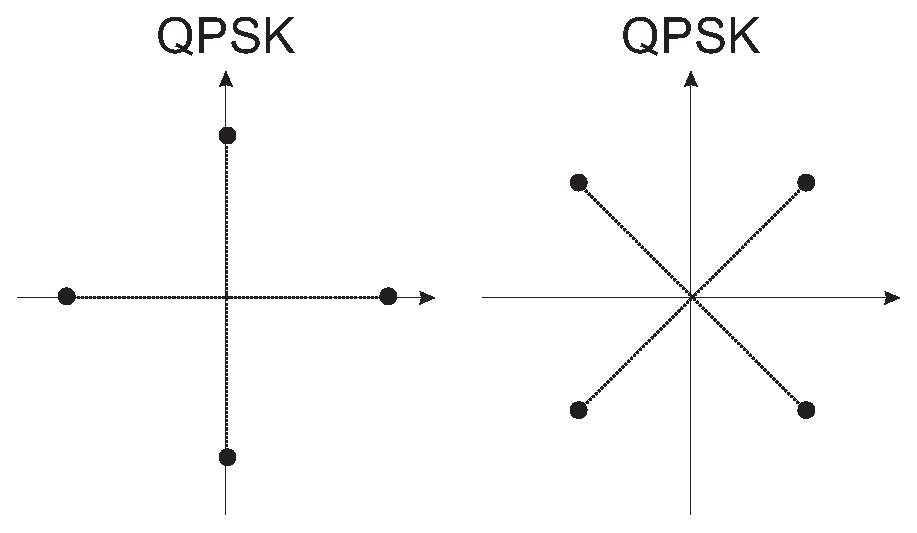
\includegraphics[width=0.6\textwidth]{../images/QPSK-signalSpaceDiagram.eps}
  }
  \centerline{(b)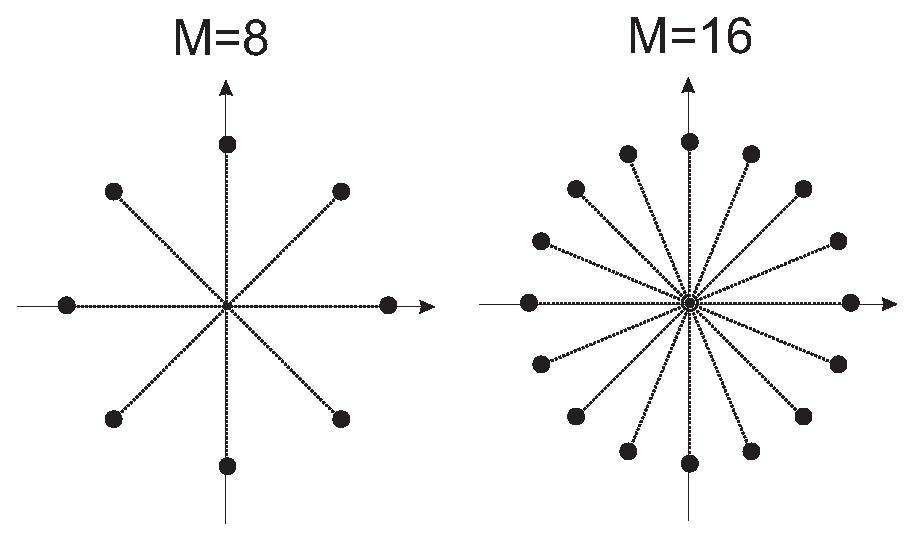
\includegraphics[width=0.6\textwidth]{../images/MPSK-signalSpaceDiagram.eps} }
  \centerline{(c)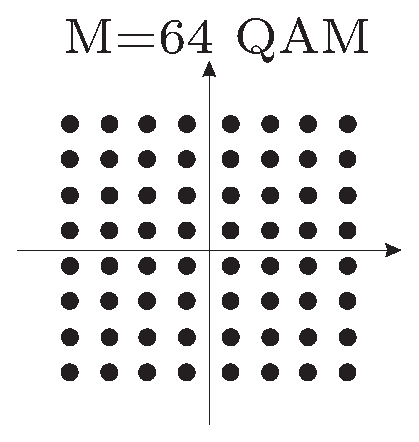
\includegraphics[width=0.3\textwidth]{../images/QAM64Eg.eps} }
  \caption{Signal constellations for (a) $M=4$ PSK (a.k.a. BPSK), (b) $M=8$ and $M=16$ PSK, and (c) 64-QAM.}
  \label{F:MPSKEg}
\end{figure}

In the next lecture we will talk about how a receiver is able to separate the received signal into components, each corresponding to one of the orthogonal waveforms $\phi_k(t)$.  From this separation, it will be able to decide which symbol was sent.


\subsection{How to Choose a Modulation}

A \textit{digital modulation} is the choice of: (1) the  linear combinations $\mbs_0, \ldots, \mbs_{M-1}$ and, (2) the orthogonal waveforms $\phi_0(t), \ldots, \phi_{K-1}(t)$.  We will choose a digital modulation as a tradeoff between the following characteristics:
\begin{enumerate}
 \item Bandwidth efficiency: How many bits per second (bps) can be sent per Hertz of signal bandwidth.  Thus the bandwidth efficiency has units of bps/Hz.
 \item Power efficiency: How much energy per bit is required at the receiver in order to achieve a desired fidelity (low bit error rate).  We typically use $S/N$ or $E_s/N_0$ or $E_b/N_0$ as our figure of merit.  This will be a major topic of the 2nd part of this course.
 \item Cost of implementation:  Things like symbol and carrier synchronization, and linear transmitters, require additional device cost, which might be unacceptable in a particular system.
\end{enumerate}




\section{Time-Domain Concept Review}

\subsection{Periodicity}

\Definition{Periodic (continuous-time)}{A signal $x(t)$ is periodic if $x(t) =
x(t+T_0)$ for some constant $T_0 \neq 0$ for all $t\in \mR$. The
smallest such constant $T_0>0$ is the \emph{period}.}

If a signal is not periodic it is {\it aperiodic}.

Periodic signals have Fourier series representations, as defined in Rice Ch.~2.


\Definition{Periodic (discrete-time)}{A DT signal $x(n)$ is periodic if $x(n) = x(n+N_0)$ for some integer
$N_0\neq 0$, for all integers $n$.  The smallest positive integer 
$N_0$ is the period.}


\subsection{Impulse Functions}

\Definition{Impulse Function}{The (Dirac) impulse function
$\delta(t)$ is the function which makes
\begin{equation} \label{E:impulseFunctionDefn}
  \int_{-\infty}^\infty x(t)\delta(t) dt = x(0)
\end{equation}
 true for any function $x(t)$ which is continuous at $t=0$.}

We are defining a function by its most important property, the
`sifting property'.  Is the following definition more
familiar?
\[
  \delta(t) = \lim_{T\rightarrow 0} \pdfarray{1/(2T)}{-T \le t \le T}
\]
You can visualize $\delta(t)$ here as an infinitely high,
infinitesimally wide pulse at the origin, with area one.  This is
why it `pulls out' the value of $x(t)$ in the integral in
(\ref{E:impulseFunctionDefn}).

Other properties of the impulse function:
\begin{itemize}
  \item Time scaling,
  \item Symmetry,
  \item Sifting at arbitrary time $t_0$,
\end{itemize}

The continuous-time unit step function is
\[
 u(t) = \pdfarray{1}{t\ge 0}
\]


\Example{Sifting Property} What is $\int_{-\infty}^\infty \frac{\sin
(\pi t)}{\pi t} \delta(1-t) dt$?

\Solution{The integral pulls out the value of the fraction when the argument of the $\delta $ function is zero, in this case, when $t=1$.  Thus plug in $t=1$ into $\frac{\sin
(\pi t)}{\pi t}$ and get $\frac{\sin
(\pi)}{\pi} = 0/\pi = 0$.}

The discrete-time impulse function (also called the Kronecker delta
or $\delta_K$) is defined as:
\[
 \delta(n) = \pdfarray{1}{n=0}
\]
(There is no need to get complicated with the math; this is well
defined.)  Also,
\[
 u(n) = \pdfarray{1}{n\ge 0}
\]





